\section{Dữ liệu}
\label{sec:data}

\subsection{Dữ liệu viễn thám Sentinel}

Việc lựa chọn ảnh vệ tinh tuân theo các tiêu chí nhằm đảm bảo chất lượng dữ liệu đầu vào. Đối với ảnh Sentinel-2, nghiên cứu sử dụng sản phẩm \textit{S2\_SR\_HARMONIZED} (Surface Reflectance Level-2A đã hiệu chỉnh) từ Google Earth Engine, ưu tiên các ảnh trong mùa khô (tháng 1--3) để giảm thiểu ảnh hưởng của mây và đảm bảo tính so sánh giữa hai thời kỳ. Mặt nạ mây được tạo từ bộ sưu tập \textit{S2\_CLOUD\_PROBABILITY} với ngưỡng xác suất 50\% để loại bỏ các điểm ảnh bị mây che phủ. Đối với ảnh Sentinel-1, sử dụng sản phẩm \textit{S1\_GRD} đã được tiền xử lý bởi ESA, các cảnh được chọn có thời gian thu nhận gần nhất với ảnh Sentinel-2 tương ứng (trong phạm vi ±7 ngày) để đảm bảo tính đồng bộ về thời gian.

\begin{table}[H]
\centering
\caption{Tổng quan dữ liệu sử dụng}
\label{tab:data_overview}
\begin{tabular}{|l|c|c|c|}
\hline
\textbf{Nguồn dữ liệu} & \textbf{Độ phân giải} & \textbf{Kỳ ảnh} &  \textbf{Số lượng} \\
\hline
Sentinel-2 trước & 10m & 30/01/2024 & 7 kênh \\
\hline
Sentinel-2 sau & 10m & 28/02/2025 & 7 kênh \\
\hline
Sentinel-1 trước & 10m & 04/02/2024 & 2 kênh \\
\hline
Sentinel-1 sau & 10m & 22/02/2025 & 2 kênh \\
\hline
Dữ liệu thực địa & - & - & 2,630 điểm \\
\hline
Ranh giới lâm nghiệp & - & - & Vector \\
\hline
\end{tabular}
\end{table}

\subsection{Thu thập dữ liệu trên Google Earth Engine}

Toàn bộ dữ liệu ảnh vệ tinh được thu thập và xử lý trên nền tảng Google Earth Engine — một hệ thống điện toán đám mây cho phép truy cập và xử lý khối lượng lớn dữ liệu viễn thám. Việc sử dụng GEE mang lại nhiều ưu điểm: truy cập trực tiếp kho dữ liệu Sentinel đã được hiệu chỉnh, khả năng xử lý dữ liệu nhanh chóng trên hạ tầng đám mây, và đảm bảo tính nhất quán trong quy trình xử lý.

Dữ liệu Sentinel-2 được truy xuất từ bộ dữ liệu \textit{COPERNICUS/S2\_SR\_HARMONIZED} — sản phẩm đã được hiệu chỉnh khí quyển và đồng nhất hóa giữa các cảm biến Sentinel-2A và 2B. Quy trình xử lý bắt đầu bằng việc lọc theo không gian và thời gian để chọn các cảnh phủ khu vực nghiên cứu trong ngày chỉ định, sau đó loại bỏ mây sử dụng bộ sưu tập \textit{S2\_CLOUD\_PROBABILITY} với ngưỡng xác suất 50\%. Tiếp theo, 4 kênh phổ cần thiết (B4-Red, B8-NIR, B11-SWIR1, B12-SWIR2) được trích xuất, chuyển đổi sang giá trị phản xạ và tính toán 3 chỉ số thực vật NDVI, NBR, NDMI. Cuối cùng, các tiles được mosaic để tạo ảnh liền mạch phủ toàn bộ khu vực nghiên cứu.

Việc lựa chọn bốn kênh phổ B4, B8, B11 và B12 trong số 13 kênh của Sentinel-2 dựa trên cơ sở khoa học về đặc tính phản xạ phổ của thực vật và yêu cầu tính toán các chỉ số thực vật phục vụ giám sát biến động rừng. Kênh B4 ở vùng ánh sáng đỏ (665 nm) ghi nhận vùng hấp thụ mạnh của diệp lục, do đó nhạy cảm với sự thay đổi hàm lượng diệp lục khi thực vật bị stress hoặc chết đi \citeen{lillesand2015}. Kênh B8 ở vùng cận hồng ngoại (842 nm) phản ánh cấu trúc mô thịt lá với phản xạ cao ở thực vật khỏe mạnh, là thành phần không thể thiếu trong hầu hết các chỉ số thực vật \citeen{rouse1974}. Hai kênh SWIR bao gồm B11 (1610 nm) và B12 (2190 nm) nhạy cảm với hàm lượng nước trong lá và cellulose, lignin trong cấu trúc thực vật, đặc biệt hiệu quả trong phát hiện các vùng rừng bị suy thoái hoặc chặt phá \citeen{key2006, gao1996}. Các kênh vùng nhìn thấy B2 và B3 không được sử dụng vì dễ bị ảnh hưởng bởi tán xạ khí quyển và không cung cấp thông tin bổ sung đáng kể so với B4 trong bối cảnh giám sát rừng. Các kênh Red Edge (B5, B6, B7) và B8a có độ phân giải không gian 20m, thấp hơn so với 10m của B4 và B8, đồng thời thông tin từ các kênh này đã được phản ánh gián tiếp qua sự kết hợp B4-B8 trong chỉ số NDVI. Nghiên cứu của Khatami et al. \citeen{khatami2016} chỉ ra rằng việc sử dụng quá nhiều kênh phổ có thể dẫn đến hiện tượng thừa thông tin mà không cải thiện độ chính xác phân loại.

Về các chỉ số thực vật, nghiên cứu sử dụng ba chỉ số NDVI, NBR và NDMI dựa trên nguyên tắc mỗi chỉ số khai thác một khía cạnh khác nhau của trạng thái thực vật, tạo ra tập đặc trưng bổ sung cho nhau mà không gây dư thừa. NDVI được lựa chọn vì là chỉ số có tính ổn định cao trong đánh giá mật độ và sức khỏe thực vật \citeen{rouse1974, huang2021}. NBR được thiết kế đặc biệt cho phát hiện biến động rừng, với độ nhạy cao đối với sự thay đổi cấu trúc tán lá khi rừng bị chặt phá hoặc cháy \citeen{key2006}. NDMI cung cấp thông tin về hàm lượng nước trong tán lá, có khả năng phát hiện stress thực vật trước khi biểu hiện rõ ràng qua NDVI \citeen{gao1996}. Các chỉ số khác như EVI (Enhanced Vegetation Index) yêu cầu kênh Blue vốn nhạy cảm với tán xạ khí quyển và ưu điểm chính của nó không vượt trội đáng kể so với NDVI trong bối cảnh rừng ngập mặn. SAVI (Soil Adjusted Vegetation Index) được thiết kế cho vùng có độ phủ thực vật thưa, trong khi rừng ngập mặn Cà Mau có độ che phủ dày đặc khiến chỉ số này không phù hợp. GNDVI sử dụng kênh Green thay cho Red nhưng thông tin này đã được phản ánh qua NDVI. Như vậy, bộ ba chỉ số NDVI, NBR và NDMI tạo thành tổ hợp tối ưu về mặt thông tin, đảm bảo tính bổ sung mà không gây dư thừa đặc trưng cho mô hình học sâu.

Dữ liệu Sentinel-1 được truy xuất từ bộ sưu tập \textit{COPERNICUS/S1\_GRD} — sản phẩm đã được tiền xử lý bởi ESA bao gồm: hiệu chỉnh quỹ đạo, loại bỏ nhiễu biên và nhiễu nhiệt, hiệu chỉnh bức xạ và hiệu chỉnh địa hình sử dụng DEM SRTM. Quy trình xử lý bổ sung bao gồm: lọc theo thời gian (±7 ngày so với Sentinel-2), chọn chế độ Interferometric Wide (IW) với quỹ đạo đi xuống, và trích xuất hai kênh VV và VH (đơn vị dB).

Việc lựa chọn cặp phân cực VV và VH dựa trên cơ chế tán xạ sóng vi ba khi tương tác với thảm thực vật rừng. Phân cực VV (phát và thu sóng theo phương thẳng đứng) nhạy cảm với tán xạ bề mặt, phản ánh đặc tính của lớp đất hoặc mặt nước bên dưới tán rừng, đặc biệt hữu ích trong việc phát hiện thay đổi độ ẩm đất sau khi rừng bị chặt phá \citeen{torres2012}. Trong khi đó, phân cực VH (phát sóng thẳng đứng, thu sóng ngang) phát sinh chủ yếu từ quá trình tán xạ thể tích trong cấu trúc tán lá và thân cây, do đó nhạy cảm đặc biệt với sự thay đổi sinh khối và mật độ tán rừng khi xảy ra chặt phá hoặc suy thoái \citeen{reiche2018}. Sự kết hợp hai phân cực này cung cấp thông tin bổ sung về cả lớp bề mặt và cấu trúc thể tích của rừng, cho phép phân biệt tốt hơn giữa các loại biến động. Các phân cực khác không được sử dụng vì chế độ IW của Sentinel-1 cho vùng đất liền nhiệt đới chỉ cung cấp cặp phân cực VV-VH theo cấu hình tiêu chuẩn của ESA \citeen{esa2024s1}, đồng thời cặp phân cực này đã được chứng minh hiệu quả trong nhiều nghiên cứu giám sát rừng nhiệt đới trước đó.

Sau khi xử lý, dữ liệu được xuất ra định dạng GeoTIFF với độ phân giải 10m và hệ quy chiếu EPSG:32648 (WGS 84 / UTM Zone 48N). Hình~\ref{fig:features_t1} và~\ref{fig:features_t2} minh họa trực quan các dữ liệu quang học (B4, B8, B11, B12), các chỉ số thực vật (NDVI, NDMI, NBR) và dữ liệu ra-đa (VV, VH) cho hai thời điểm trước và sau biến động.

% Figure cho T1 (Kỳ trước)
\begin{figure}[H]
\centering
\begin{subfigure}[b]{0.32\textwidth}
    \includegraphics[width=\textwidth]{chapter2/T1-B4.png}
    \caption{B4 (Red)}
\end{subfigure}
\hfill
\begin{subfigure}[b]{0.32\textwidth}
    \includegraphics[width=\textwidth]{chapter2/T1-B8.png}
    \caption{B8 (NIR)}
\end{subfigure}
\hfill
\begin{subfigure}[b]{0.32\textwidth}
    \includegraphics[width=\textwidth]{chapter2/T1-B11.png}
    \caption{B11 (SWIR1)}
\end{subfigure}

\begin{subfigure}[b]{0.32\textwidth}
    \includegraphics[width=\textwidth]{chapter2/T1-B12.png}
    \caption{B12 (SWIR2)}
\end{subfigure}
\hfill
\begin{subfigure}[b]{0.32\textwidth}
    \includegraphics[width=\textwidth]{chapter2/T1-NDVI.png}
    \caption{NDVI}
\end{subfigure}
\hfill
\begin{subfigure}[b]{0.32\textwidth}
    \includegraphics[width=\textwidth]{chapter2/T1-NDMI.png}
    \caption{NDMI}
\end{subfigure}

\begin{subfigure}[b]{0.32\textwidth}
    \includegraphics[width=\textwidth]{chapter2/T1-NBR.png}
    \caption{NBR}
\end{subfigure}
\hfill
\begin{subfigure}[b]{0.32\textwidth}
    \includegraphics[width=\textwidth]{chapter2/T1-VV.png}
    \caption{VV (SAR)}
\end{subfigure}
\hfill
\begin{subfigure}[b]{0.32\textwidth}
    \includegraphics[width=\textwidth]{chapter2/T1-VH.png}
    \caption{VH (SAR)}
\end{subfigure}
\caption{Các kênh quang học, chỉ số thực vật và dữ liệu ra-đa kỳ trước (T1 - 01/2024)}
\label{fig:features_t1}
\end{figure}

% Figure cho T2 (Kỳ sau)
\begin{figure}[H]
\centering
\begin{subfigure}[b]{0.32\textwidth}
    \includegraphics[width=\textwidth]{chapter2/T2-B4.png}
    \caption{B4 (Red)}
\end{subfigure}
\hfill
\begin{subfigure}[b]{0.32\textwidth}
    \includegraphics[width=\textwidth]{chapter2/T2-B8.png}
    \caption{B8 (NIR)}
\end{subfigure}
\hfill
\begin{subfigure}[b]{0.32\textwidth}
    \includegraphics[width=\textwidth]{chapter2/T2-B11.png}
    \caption{B11 (SWIR1)}
\end{subfigure}

\begin{subfigure}[b]{0.32\textwidth}
    \includegraphics[width=\textwidth]{chapter2/T2-B12.png}
    \caption{B12 (SWIR2)}
\end{subfigure}
\hfill
\begin{subfigure}[b]{0.32\textwidth}
    \includegraphics[width=\textwidth]{chapter2/T2-NDVI.png}
    \caption{NDVI}
\end{subfigure}
\hfill
\begin{subfigure}[b]{0.32\textwidth}
    \includegraphics[width=\textwidth]{chapter2/T2-NDMI.png}
    \caption{NDMI}
\end{subfigure}

\begin{subfigure}[b]{0.32\textwidth}
    \includegraphics[width=\textwidth]{chapter2/T2-NBR.png}
    \caption{NBR}
\end{subfigure}
\hfill
\begin{subfigure}[b]{0.32\textwidth}
    \includegraphics[width=\textwidth]{chapter2/T2-VV.png}
    \caption{VV (SAR)}
\end{subfigure}
\hfill
\begin{subfigure}[b]{0.32\textwidth}
    \includegraphics[width=\textwidth]{chapter2/T2-VH.png}
    \caption{VH (SAR)}
\end{subfigure}
\caption{Các kênh phổ quang học, chỉ số thực vật và dữ liệu ra-đa kỳ sau (T2 - 02/2025)}
\label{fig:features_t2}
\end{figure}

\subsection{Dữ liệu thực địa tại Cà Mau}

Dữ liệu thực địa được Công ty TNHH Tư vấn và Phát triển Đồng Xanh (GFD) thu thập trong khuôn khổ thực hiện đề tài ``Ứng dụng công nghệ viễn thám, ảnh vệ tinh để quản lý, giám sát tài nguyên rừng và sạt lở ven biển trên địa bàn tỉnh Cà Mau'' \citevi{gfd2025} và được cung cấp cho nghiên cứu này. Quy trình thu thập gồm ba giai đoạn. Giai đoạn đầu tiên là khảo sát thực địa bằng thiết bị bay không người lái (drone) để ghi nhận hình ảnh và xác định trạng thái rừng. Giai đoạn thứ hai là số hóa các điểm dữ liệu thực địa trên phần mềm QGIS, đối chiếu với ảnh vệ tinh Sentinel-2. Giai đoạn cuối cùng là kiểm tra chéo và loại bỏ các điểm không rõ ràng hoặc nằm trong vùng mây che phủ. Dữ liệu cuối cùng được xuất dưới dạng file CSV với cấu trúc gồm 4 trường: \textit{id}, \textit{label}, \textit{x} và \textit{y} (tọa độ theo hệ quy chiếu EPSG:32648).

\begin{table}[H]
\centering
\caption{Thống kê dữ liệu thực địa theo lớp biến động}
\label{tab:ground_truth}
\begin{tabular}{|c|l|c|c|l|}
\hline
\textbf{Lớp} & \textbf{Tên} & \textbf{Số điểm} & \textbf{Tỷ lệ} & \textbf{Mô tả} \\
\hline
0 & Rừng ổn định & 656 & 24,9\% & Có rừng ở cả 2 kỳ \\
\hline
1 & Mất rừng & 650 & 24,7\% & Có rừng $\rightarrow$ không có rừng \\
\hline
2 & Phi rừng ổn định & 664 & 25,3\% & Không có rừng ở cả 2 kỳ \\
\hline
3 & Phục hồi rừng & 660 & 25,1\% & Không có $\rightarrow$ có rừng \\
\hline
\textbf{Tổng} & & \textbf{2.630} & \textbf{100\%} & Phân bố cân bằng \\
\hline
\end{tabular}
\end{table}

Phân bố không gian của các điểm dữ liệu thực địa được minh họa trong Hình~\ref{fig:ground_truth_map}. Các điểm mẫu được thu thập phân tán trên toàn bộ khu vực nghiên cứu, đảm bảo tính đại diện về mặt không gian cho các loại hình biến động rừng khác nhau.

\begin{figure}[H]
\centering
\includegraphics[width=0.9\textwidth]{chapter3/samples.png}
\caption{Bản đồ phân bố không gian các điểm dữ liệu thực địa trên khu vực nghiên cứu tỉnh Cà Mau}
\label{fig:ground_truth_map}
\end{figure}

Mỗi điểm ảnh trong bộ dữ liệu được biểu diễn bởi 27 đặc trưng: 9 đặc trưng tại thời điểm $T_1$, 9 đặc trưng tại thời điểm $T_2$, và 9 đặc trưng delta ($\Delta = T_2 - T_1$). Mô hình CNN sử dụng toàn bộ 27 đặc trưng này làm đầu vào để tận dụng tối đa thông tin từ cả hai thời điểm quan sát. Tuy nhiên, để phân tích trực quan khả năng phân biệt của dữ liệu, nghiên cứu lựa chọn minh họa 9 đặc trưng delta thông qua (Hình~\ref{fig:pairplot_delta}). Việc lựa chọn này xuất phát từ hai lý do chính. Thứ nhất, biểu đồ Phân bố với 27 đặc trưng sẽ tạo ra ma trận $27 \times 27 = 729$ ô, quá lớn để quan sát và phân tích hiệu quả. Thứ hai, đặc trưng delta trực tiếp biểu diễn sự thay đổi giữa hai thời điểm, do đó phù hợp nhất để đánh giá khả năng phân tách các lớp biến động rừng.

\begin{figure}[H]
\centering
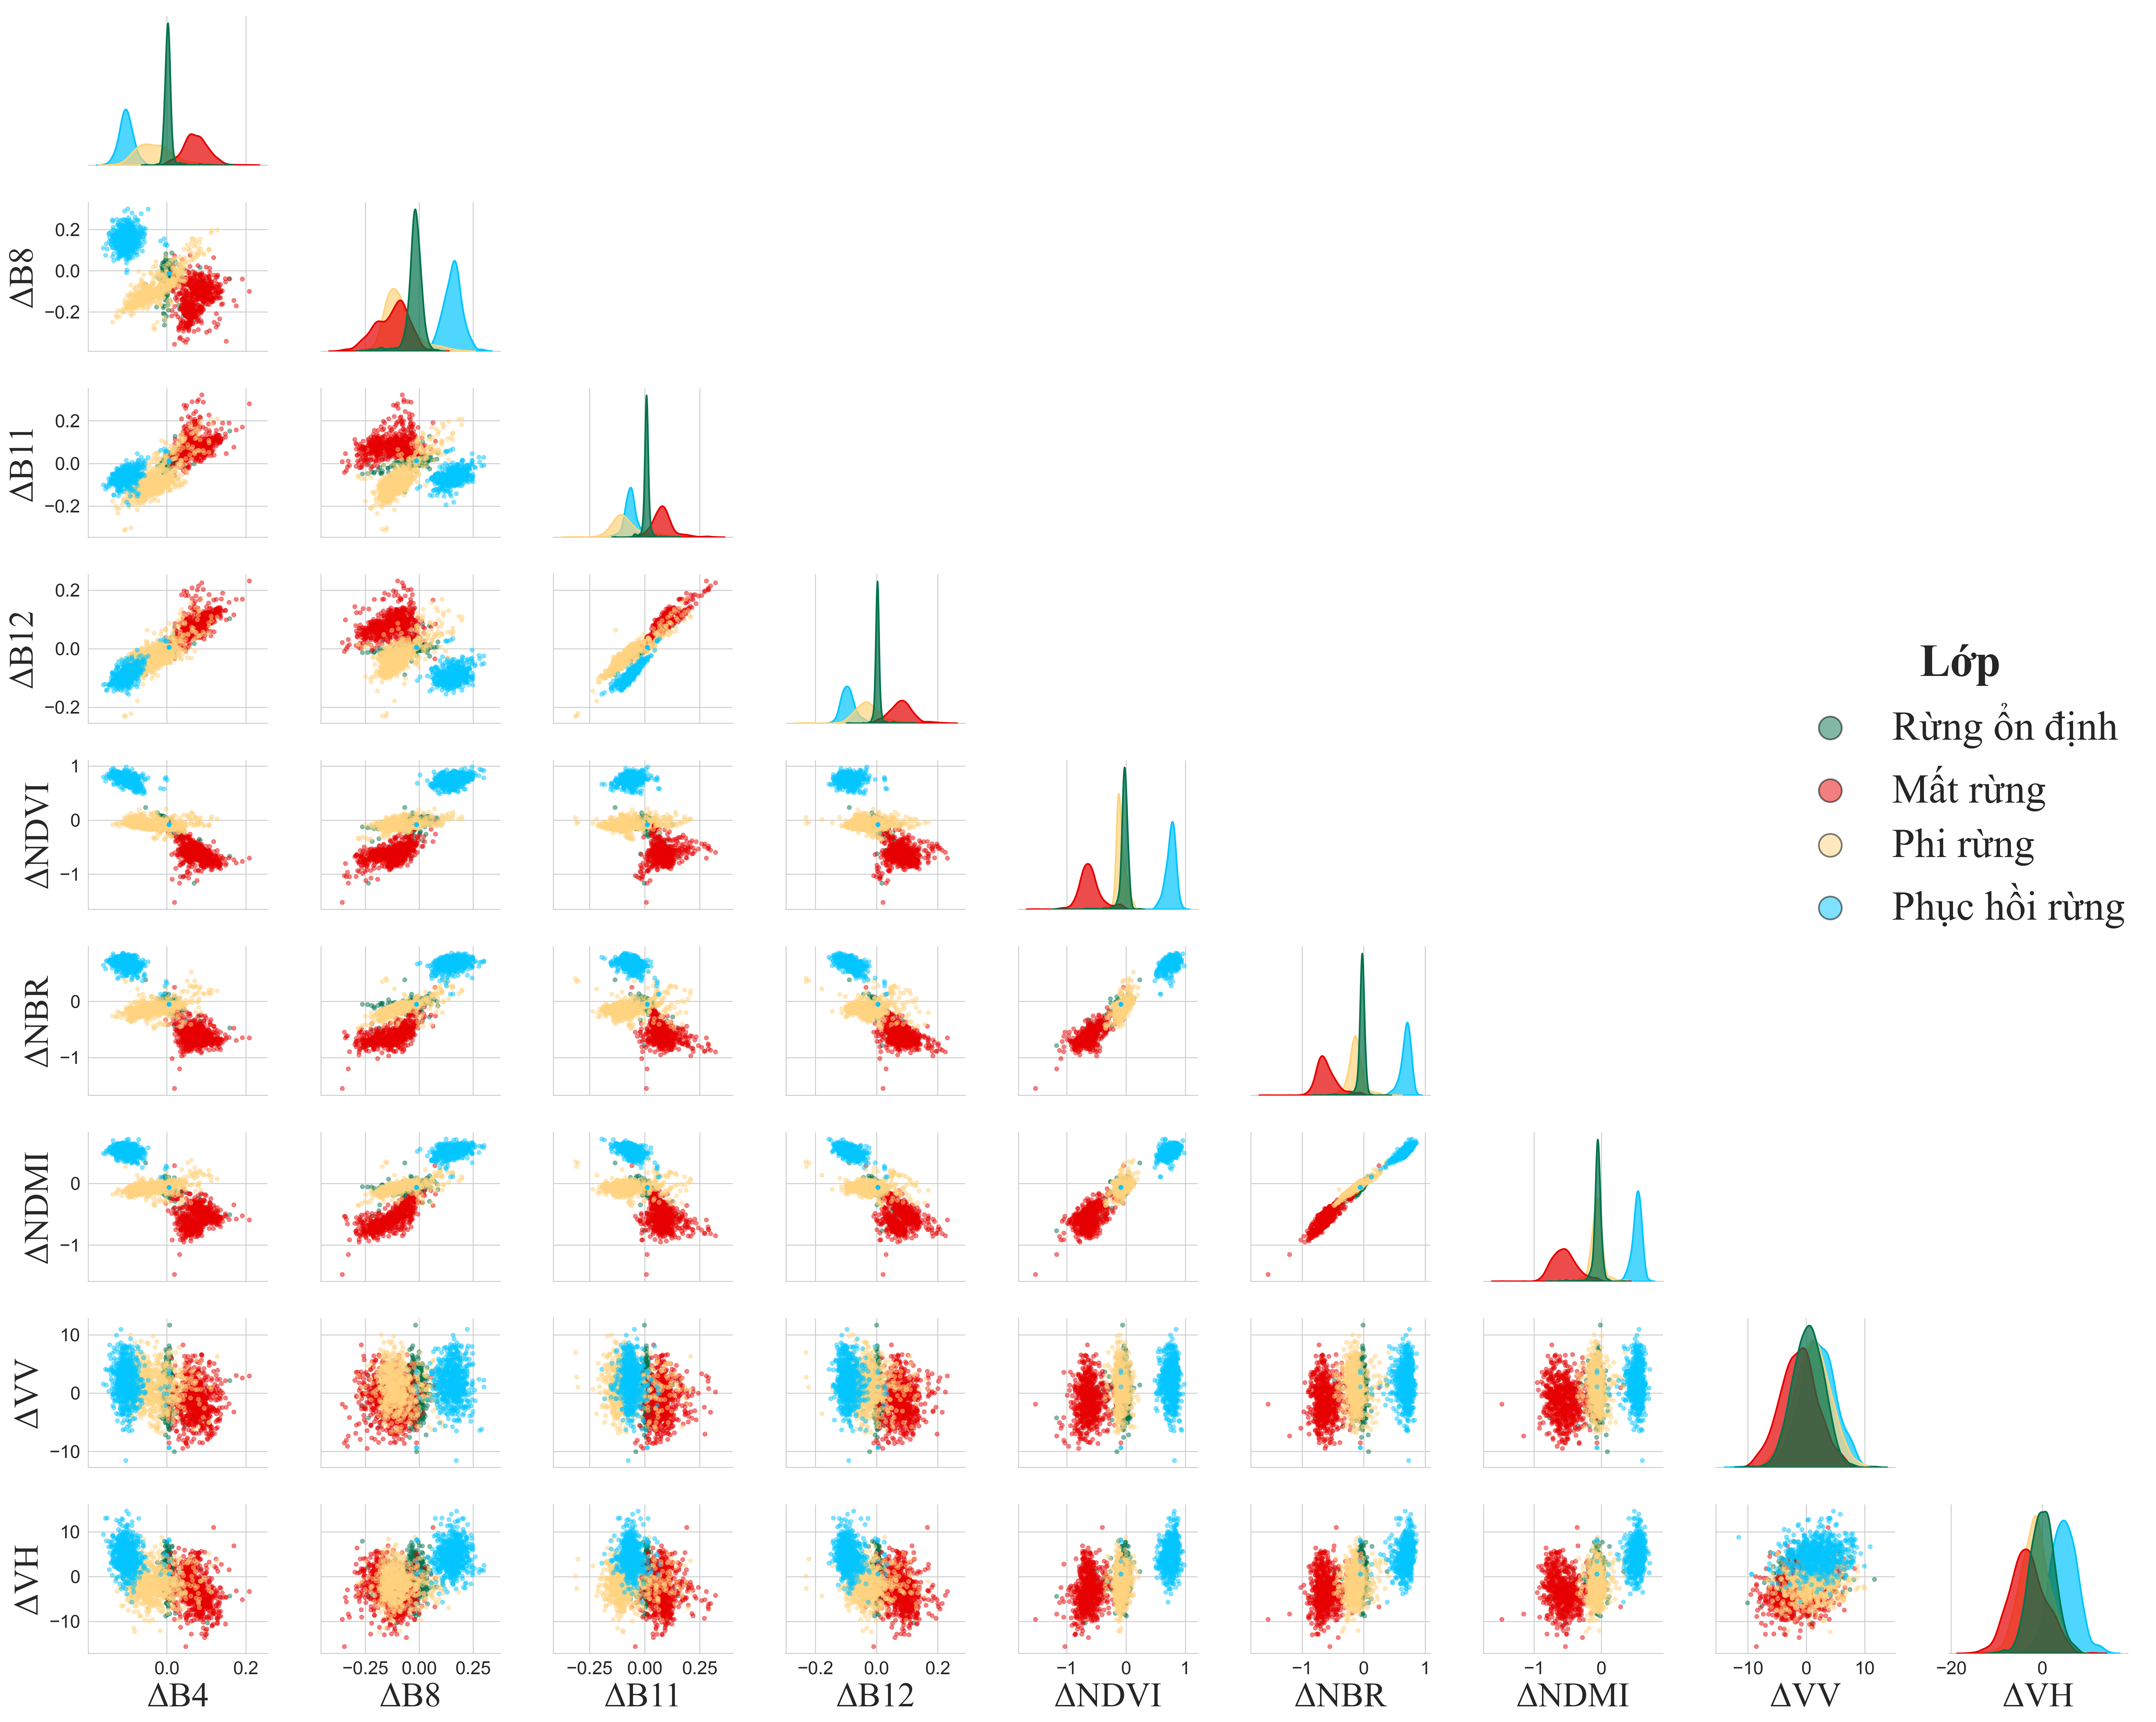
\includegraphics[width=0.95\textwidth]{img/chapter3/pairplot_delta_features.png}
\caption{Phân bố các đặc trưng delta theo lớp biến động rừng}
\label{fig:pairplot_delta}
\end{figure}

Biểu đồ trình bày mối quan hệ giữa 9 đặc trưng delta bao gồm các band quang phổ Sentinel-2 ($\Delta$B4, $\Delta$B8, $\Delta$B11, $\Delta$B12), các chỉ số thực vật ($\Delta$NDVI, $\Delta$NBR, $\Delta$NDMI) và các kênh ra-đa Sentinel-1 ($\Delta$VV, $\Delta$VH). Trên đường chéo chính, biểu đồ thể hiện phân bố của từng đặc trưng theo bốn lớp biến động; các ô còn lại hiển thị biểu đồ tán xạ giữa các cặp đặc trưng.

Phân tích phân bố trên đường chéo cho thấy các chỉ số thực vật delta thể hiện khả năng phân biệt vượt trội giữa các lớp biến động. Cụ thể, lớp Rừng ổn định và Phi rừng có phân bố tập trung quanh giá trị 0, phản ánh sự ổn định về lớp phủ thực vật qua hai thời điểm quan sát. Ngược lại, lớp Mất rừng thể hiện phân bố lệch về phía âm do sự suy giảm các chỉ số thực vật khi rừng bị chuyển đổi, trong khi lớp Phục hồi rừng có phân bố lệch về phía dương tương ứng với sự gia tăng sinh khối thực vật. Sự phân tách rõ ràng này khẳng định vai trò then chốt của $\Delta$NDVI, $\Delta$NBR và $\Delta$NDMI trong việc nhận diện biến động rừng.

Đối với các band quang phổ gốc, mức độ chồng chéo giữa các lớp cao hơn so với các chỉ số thực vật, tuy nhiên $\Delta$B8 (kênh cận hồng ngoại) vẫn cho thấy khả năng phân biệt tương đối tốt giữa lớp Mất rừng và Phục hồi rừng. Các đặc trưng ra-đa $\Delta$VV và $\Delta$VH có phân bố chồng chéo đáng kể giữa bốn lớp, cho thấy khả năng phân biệt độc lập hạn chế hơn so với dữ liệu quang học. Tuy nhiên, việc tích hợp dữ liệu ra-đa vẫn mang lại giá trị bổ sung, đặc biệt trong điều kiện mây che phủ thường xuyên tại khu vực nghiên cứu.

Phân tích các biểu đồ tán xạ cho thấy mối tương quan dương mạnh giữa ba chỉ số thực vật ($\Delta$NDVI, $\Delta$NBR, $\Delta$NDMI), thể hiện qua sự phân bố các điểm dữ liệu gần đường chéo. Tương tự, $\Delta$B11 và $\Delta$B12 có tương quan cao do cùng thuộc dải sóng ngắn hồng ngoại (SWIR). Trên không gian đặc trưng hai chiều của các chỉ số thực vật, lớp Mất rừng và Phục hồi rừng phân bố ở hai vùng đối lập nhau, trong khi lớp Rừng ổn định và Phi rừng tập trung quanh gốc tọa độ. Đặc điểm phân bố này tạo điều kiện thuận lợi cho mô hình CNN trong việc học các ranh giới quyết định phân tách bốn lớp biến động.
